% Written by ../code/make_numbers.py. Do not edit by hand.
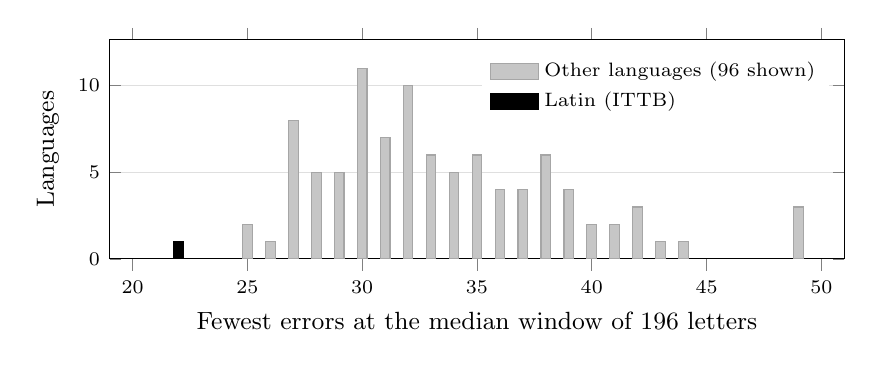
\begin{tikzpicture}
\begin{axis}[width=0.9\linewidth, height=0.36\linewidth, ybar=0pt, bar width=3.5pt, bar shift=0pt,
  xmin=19, xmax=51, ymin=0, enlarge y limits={upper, value=0.15},
  xlabel={Fewest errors at the median window of 196 letters}, ylabel={Languages},
  label style={font=\small}, ticklabel style={font=\scriptsize}, ymajorgrids, grid style={gray!25},
  legend style={font=\scriptsize, draw=none, at={(0.98,0.95)}, anchor=north east}, legend cell align=left, area legend]
\addplot[fill=gray!45, draw=gray!70] coordinates {(25,2) (26,1) (27,8) (28,5) (29,5) (30,11) (31,7) (32,10) (33,6) (34,5) (35,6) (36,4) (37,4) (38,6) (39,4) (40,2) (41,2) (42,3) (43,1) (44,1) (49,3)};
\addlegendentry{Other languages (96 shown)}
\addplot[fill=black, draw=black] coordinates {(22,1)};
\addlegendentry{Latin (ITTB)}
\end{axis}
\end{tikzpicture}
